\chapter{Mass segregation trends in SDSS galaxy groups}
\label{chap:massSeg}

\section{Introduction}
\label{sec:intro_ms}

It has been well established that galaxy properties dpend strongly on
local environment \citep[e.g.][]{oemler1974, hogg2004, blanton2005b,
  tal2014}.  Galaxies in dense environments such as clusters tend to
have lower star formation rates (SFRs), while isolated field galaxies
are generally actively forming stars \citep[e.g.][]{balogh2000,
  ball2008, wetzel2012}.  It is also well known that galaxy
properties, such as SFR, depend strongly on galaxy mass
\citep[e.g.][]{poggianti2008}.  It is critical to study the
distribution of galaxy masses within haloes of different masses in
order to ascertain whether the variations in galaxy properties with
environment are due to physical mechanisms acting in dense
environments, or simply due to the fact that high-density environments
contain more high-mass galaxies.  Intermediate-density environments,
galaxy groups, represent not only the most common environment in the
local Universe \citep{geller1983, eke2005}, but also represent the
environment where many physical processes are efficient.  Galaxy
interactions such as mergers and harassment are favoured in this
environment because of the low relative velocities between galaxies
\citep{zabludoff1998, brough2006}.
\par
The study of mass segregation in groups can be used to elucidate
information on physical processes such as dynamical friction, galaxy
mergers, and tidal stripping.  Mass segregation in bound structures
has generally been predicted as a result of dynamical friction
\citep{chandrasekhar1943}.  Dynamical friction acts as a drag force on
orbiting bodies and massive galaxies within groups and clusters are
expected to migrate to smaller radii as time progresses.  If dynamical
friction is a dominant factor, then clear mass segregation should be
observed in evolved groups and clusters.
\par
Galaxy groups are not static systems, but are constantly being
replenished by infalling galaxies from the field.  Infalling galaxies
are preferentially found at large radii \citep{wetzel2013} and the
difference in stellar mass distributions between evolved group members
and infalling galaxies could affect the strength of mass segregation.
\par
If significant mass segregation is not found, then this implies that
either: the time-scale associated with dynamical friction is greater
than the age of the group/cluster, or that there are other physical
processes, such as merging, tidal stripping, or pre-processing, which
are playing a more important role than dynamical friction.
\par
Recent work has shown conflicting results with regards to the presence
of mass segregation in groups and clusters.  \citet{ziparo2013} find
no evidence for strong mass segregation in X-ray selected groups out
to $z=1.6$, for a sample of galaxies with $M_\mathrm{star} >
10^{10.3}\Msun$.  \citet{vonderlinden2010} examine Sloan Digital Sky
Survey (SDSS) galaxy clusters and find no evidence for mass
segregation in four different redshift bins at $z < 0.1$.  von der
Linden et al. make redshift-dependent stellar mass cuts ranging from
$10^{9.6}$ to $10^{10.5}\Msun$.  \citet{vulcani2013} use mass-limited
samples at $0.3 \le z \le 0.8$ from the IMACS Cluster Building Survey
and the ESO Distant Cluster Survey, with stellar mass cuts at
$M_\mathrm{star} > 10^{10.5}\Msun$ and $M_\mathrm{star} >
10^{10.2}\Msun$, respectively, to study galaxy stellar mass functions
in different environments.  Vulcani et al. find no statistical
differences between mass functions of galaxies located at different
cluster-centric distances.
\par
Conversely, \citet{balogh2014} find evidence for mass segregation in
Group Environment Evolution Collaboration 2 (GEEC2) groups at $0.8 < z
< 1$, using as stellar-mass-limited sample with $M_\mathrm{star} >
10^{10.3}\Msun$.  Using a volume limited sample of zCOSMOS groups,
\citet{presotto2012} find evidence for mass segregation in their whole
sample at both $0.2 \le z \le 0.45$ and $0.45 \le z \le 0.8$.
Presotto et al. also break their sample into rich and poor groups at
$0.2 \le z \le 0.45$, and find evidence for mass segregation within
rich groups but find no evidence for mass segregation within poor
groups.  Using a $V_\mathrm{max}$-weighted sample with a stellar mass
cut at $10^{9.0}\Msun$, \citet{vandenbosch2008} find evidence for mass
segregation in SDSS groups.
\par
It is clear that there is no consensus regarding the strength of mass
segregation in groups and clusters or its halo mass dependence.
\par
In this Letter, we present evidence of the presense of a small, but
significant, amount of mass segregation in SDSS galaxy groups.  We
show that the detection of mass segregation is dependent on stellar
mass completeness, with completeness cuts at relatively high stellar
masses potentially masking underlying mass segregation trends.  We
also show that the strength of mass segregation scales inversely with
halo mass, with cluster-sized haloes showing little to no observable
mass segregation.  In Section~\ref{sec:data_ms}, we briefly describe
our data set, 
in Section~\ref{sec:results_ms} we present our results from this work,
in Section
... we provide a discussion of our results, and in Section ... we give
a summary of the results and make concluding statements.
\par
In this Letter, we assume a flat $\Lambda$ cold dark matter cosmology
with $\Omega_M = 0.3$, $\Omega_\Lambda = 0.7$, and $H_0 =
70\,\mathrm{km}\,\mathrm{s^{-1}}\,\mathrm{Mpc^{-1}}$.

\section{Data}
\label{sec:data_ms}

The results presented in this Letter utilize the group catalogue of
\cite{yang2007}.  This catalogue is contructed by applying the
halo-based group finder of \citet{yang2005, yang2007} to the New York
University Value-Added Galaxy Catalogue (NYU-VAGC;
\citealt{blanton2005a}), which is based on the SDSS Data Release 7
(DR7; \citealt{abazajian2009}.  Stellar masses are obtained from the
NYU-VAGC and are computed using the methodology of
\citet{blanton2007}, assuming a \citet{chabrier2003} initial mass
function.  Halo masses are determined using the ranking of the
characteristic stellar mass, $M_{\star,\mathrm{grp}}$, and assuming a
relationship between $M_\mathrm{halo}$ and $M_{\star,\mathrm{grp}}$
\citep{yang2007}.  $M_{\star,\mathrm{grp}}$ is defined by Yang et
al. as

\begin{equation}
  M_{\star,\mathrm{grp}} = \frac{1}{g(L_{19.5},\,L_\mathrm{lim})}
  \sum_i \frac{M_{\mathrm{star},i}}{C_i},
\end{equation}

\noindent
where $M_{\mathrm{star},i}$ is the stellar mass of the $i$th member
galaxy, $C_i$ is the completeness of the survey at the position of
that galaxy, and $g(L_{19.5},\,L_\mathrm{lim})$ is a correction factor
which accounts for galaxies missed due to the magnitude limit of the
survey.
\par
Halo-centric distance for each galaxy is not given explicitly in the
Yang catalogue; however, we calculate it using the redshift of the
group and the angular separation of the galaxy and halo centre on the
sky.  We measure group-centric radius from the luminosity-weighted
centre of each group, and normalize our grou-centric radii by
$R_{200}$.  We use the definition for $R_{200}$ as given in
\citet{carlberg1997}

\begin{equation}
  R_{200} = \frac{\sqrt{3} \sigma}{10 H(z)},
\end{equation}

\noindent
where the Hubble parameter, $H(z)$, is defined as

\begin{equation}
  H(z) = H_0\sqrt{\Omega_M (1+z)^3 + \Omega_\Lambda},
\end{equation}

\noindent
and we calculate the velocity dispersion, $\sigma$, as

\begin{equation}
  \sigma = 397.9\,\mathrm{km}\,\mathrm{s^{-1}} \left
(\frac{M_\mathrm{halo}}{10^{14}\,h^{-1}\Msun} \right )^{0.3214},
\end{equation}

\noindent
where the above is a fitting function given in \citet{yang2007}.
\par
For our analysis we select group galaxies with redshift, $z < 0.1$,
that are within two virial radii of the group centre, and groups with
a minimum of three galaxy members -- although our results are not
sensitive to these specific cuts.  For our sample over 95 per cent of
group galaxies reside within two virial radii of the group centre.  We
also subtract the most massive galaxy (MMG) from each group, to ensure
that any underlying radial mass trend is not contaminated by the MMG.
\par
This sample is not volume limited, therefore, the sample will suffer
from the Malmquist bias.  This leads to a bias towards objects of
higher luminosity and stellar mass, with increasing redshift.  To
account for this bias we weight our sample by $1/V_\mathrm{max}$,
where $V_\mathrm{max}$ is the comoving volume of the Universe out to a
comoving radius at which the galaxy would have met the selection
criteria for the sample.  For our $V_\mathrm{max}$ weights we apply
the values presented in the catalogue of \citet{simard2011} to our
sample.
\par
In order to investigate the effect of stellar mass limits on the
detection of mass segregation, we use samples corresponding to various
stellar mass cuts.  We perform our analysis on an unweighted sample
with two mass cuts corresponding to $M_\mathrm{star} > 10^{10.5}\Msun$
(4152 galaxies in 1970 groups) and $M_\mathrm{star} > 10^{10.0}\Msun$
(26 774 galaxies in 4534 groups); and a $V_\mathrm{max}$-weighted
sample with mass cuts at $M_\mathrm{star} > 10^{9.0}\Msun$
(56 957 galaxies in 7217 groups) and $M_\mathrm{star} > 10^{8.5}\Msun$
(59 791 galaxies in 7289 groups).  The unweighted sample is stellar
mass complete down to $M_\mathrm{star} > 10^{10.0}\Msun$.  Therefore,
for both the weighted and unweighted sample, we have two different
stellar mass cuts, giving us four separate samples in total.

\section{Results}
\label{sec:results_ms}

\subsection{Mass segregation in SDSS groups}

\begin{figure}[!ht]
  \centering
  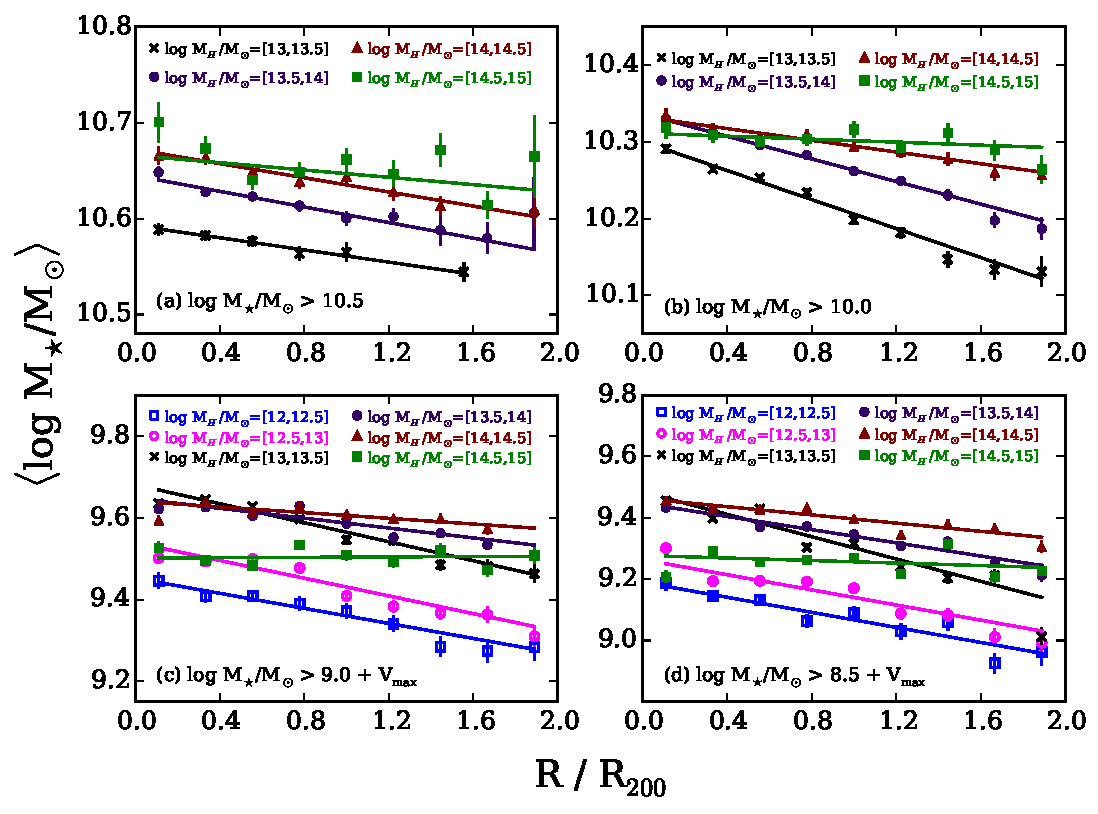
\includegraphics[width=\textwidth]{Rmass.pdf}
  \caption{All panels show mean mass as a function of normalized
    distance for various halo mass bins, with error bars corresponding
  to $1\sigma$ statistical errors.  The solid lines correspond to
  weighted least-squares fits for each halo mass bin.  Top left:
  unweighted sample, for galaxies with $\log(M_\mathrm{star}/\Msun) >
  10.5$.  Top right: unweighted sample, for galaxies with
  $\log(M_\mathrm{star}/\Msun) > 10.0$.  Bottom left:
  $V_\mathrm{max}$-weighted sample, for galaxies with
  $\log(M_\mathrm{star}/\Msun) > 9.0$.  Bottom right:
  $V_\mathrm{max}$-weighted sample, for galaxies with
  $\log(M_\mathrm{star}/\Msun) > 8.5$.  Note that different mass
  scales are used in each panel.  There are more halo mass bins in the
  bottom row due to the increased number of low-mass galaxies as a
  result of $V_\mathrm{max}$ weighting.}
  \label{fig:Rmass}
\end{figure}

In Fig.~\ref{fig:Rmass} we plot mean stellar mass as a function of
radial distance from the group centre for various halo mass bins.
Fig~\ref{fig:Rmass}(a) corresponds to our high-mass cut, unweighted
sample; Fig~\ref{fig:Rmass}(b) corresponds to our low-mass cut,
unweighted sample; Fig~\ref{fig:Rmass}(c) corresponds to our high-mass
cut, weighted sample; and Fig~\ref{fig:Rmass}(d) corresponds to our
low-mass cut, weighted sample.
\par
For all halo mass bins, and regardless of the mass cut, the unweighted
sample shows statistically significant mass segregation with a
weighted linear least-squares fit.  The $V_\mathrm{max}$-weighted
sample shows statistically significant mass segregation for the five
lower halo mass bins, whereas the highest halo mass bin has a
best-fitting slope consistent with zero -- this trend hold for both
mass cuts.  For both the weighted and unweighted samples there is a
clear trend of the slope with halo mass -- more massive haloes show
weaker mass segregation.  This result will be discussed in Section ...
\par
We find that our highest halo mass sample ($M_\mathrm{halo} >
10^{14.5}\Msun$) has a large number of low-mass galaxies when compared
to the high-halo-mass samples, which leads to a smaller mean stellar
mass in the $V_\mathrm{max}$-weighted results shown in
Figs~\ref{fig:Rmass}(c) and (d).  While this introduces a shift in
normalization, it does not affect the mass segregation trend and
therefore does not change the key result that mass segregation depends
on halo mass.

\subsection{Massive galaxy fraction}

\begin{figure}[!ht]
  \centering
  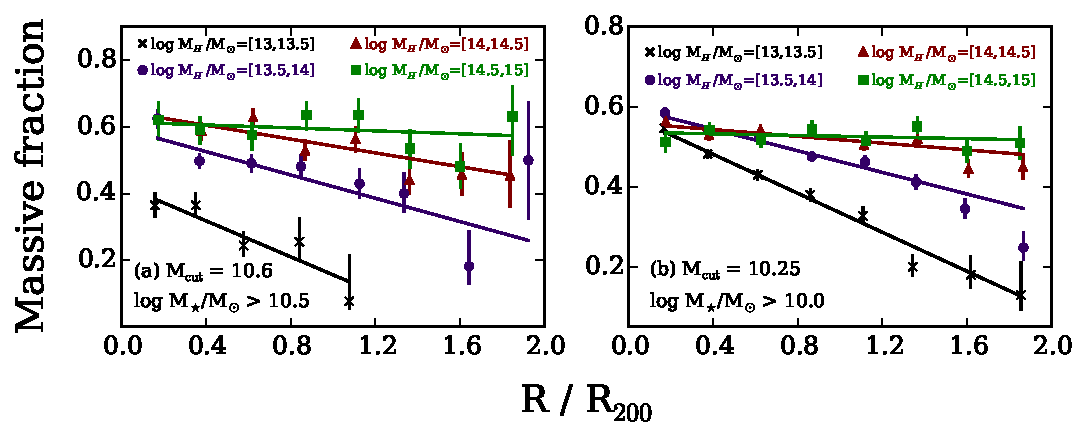
\includegraphics[width=\textwidth]{Rfrac.pdf}
  \caption{Fraction of massive galaxies with respect to normalized
    radial distance.  Error bars are given by a $1\sigma$ binomial
    confidence interval, calculated using the beta distribution as
    outlined in \citet{cameron2011}.  The solid lines correspond to
    weighted least-squares fits for each halo mass bin.  Left-hand
    panel: the fraction of galaxies with $\log(M_\mathrm{star}/\Msun)
    > 10.25$ as a function of radial distance, for the unweighted
    sample with $M_\mathrm{star} > 10^{10}\Msun$.  Right-hand panel:
    the fraction of galaxies with $\log(M_\mathrm{star}/\Msun) > 10.5$
  as a function of radial distance, for the unweighted sample with
  $M_\mathrm{star} > 10^{10}\Msun$.}
  \label{fig:Rfrac}
\end{figure}

An alternative way to investigate galaxy populations within the group
sample is to study the fraction of `massive' galaxies at various
group-centric radii.  In Fig..., we plot the fraction of massive
galaxies as a function of radial distance for two different
definitions of what constitutes a massive galaxy.  We calculate the
massive fraction for each radial bin as

\begin{equation}
  f_m(M_\mathrm{cut}) =
  \frac{\#\;\mathrm{galaxies}\;\mathrm{with}\;M_\mathrm{star} >
    M_\mathrm{cut}}{\#\;\mathrm{galaxies}\;\mathrm{with}\;M_\mathrm{star}
    > 10^{10}\Msun},
\end{equation}

\noindent
where $M_\mathrm{cut}$ is a stellar mass cut-off above which we define
a massive galaxy.  We initially apply a high-mass galaxy cut,
$M_\mathrm{cut}$, at $10^{10.25}\Msun$, corresponding to the median
stellar mass of the unweighted sample (with the low-mass cut at
$10^{10}\Msun$).  Comparing Figs~\ref{fig:Rmass}(b) and
\ref{fig:Rfrac}(a) we see essentially identical trends.  We observe
the same trends of mass segregation whether we look at the average
galaxy mass at a given radius, or consider the fraction of massive
galaxies.
\par
To confirm that this trend is robust regardless of the mass cut-off
used to define a massive galaxy, we make the same plot but now use
$M_\mathrm{cut} = 10^{10.5}\Msun$.  Comparing Figs~\ref{fig:Rfrac}(a)
and (b) we see that while the overall fractions of massive galaxies
decrease with increasing the stellar mass cut, the trend essentially
stays the same.  There is clear evidence for mass segregation and the
strength of mass segregation depends on halo mass.

% Bibliography
%
\bibliographystyle{apj}
\bibliography{masters-thesis}
